\subsection*{Hovedmenu} \label{sec:MVCHovedmenu}
Hovedmenuen er den primære grænseflade, hvor andre grænseflader kan tilgås fra via deres controller.
Hovedmenuen inddeles i en boundary samt en dertilhørende controller. Disse fremgår af \autoref{fig:Designhovedmenu}.

\begin{figure} [H]
\centering
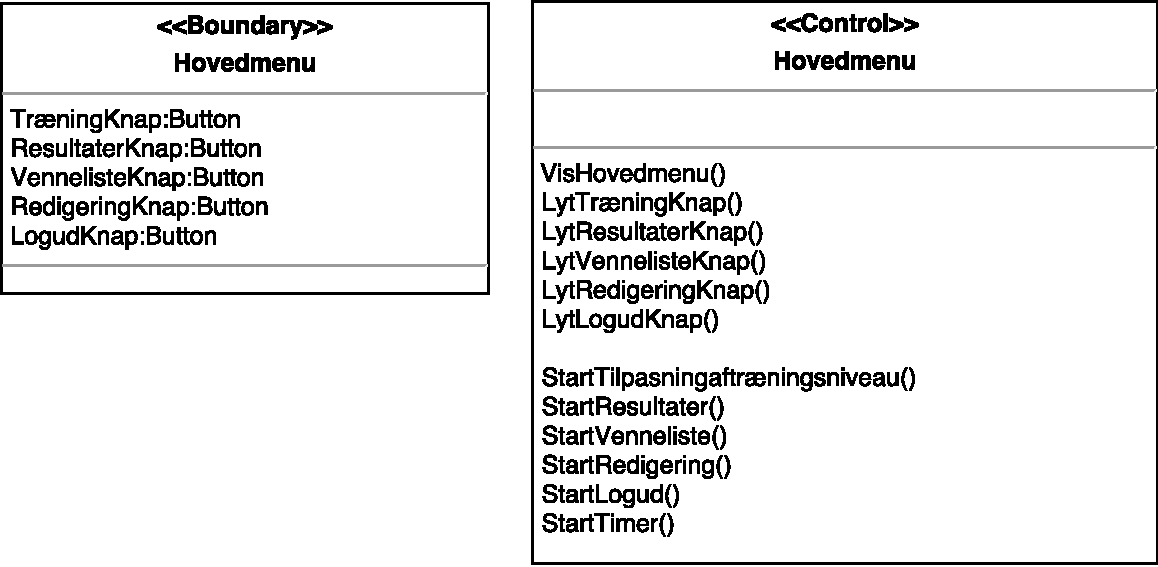
\includegraphics[width=0.9\textwidth]{figures/MVC/MVCHovedmenu}
\caption{Designklasser for hovedmenu. Til venstre ses grænsefladen og til højre tilhørende controller.}
\label{fig:Designhovedmenu}
\end{figure}

\noindent
Grænsefladen for \textit{Hovedmenu} skal tillade adgang til app'ens forskellige funktionaliteter, herunder skal det være muligt at tilgå træning, resultater, venneliste, redigering samt log ud. Funktionaliteterne tilgås via tilhørende knapper af typen Button. 

Controlleren indeholder metoderne Vis, Lyt og Start. Den viser grænsefladen for layoutet for hovedmenuen og lytter til de forskellige knapper. Et sekvensdiagram hertil er udarbejdet, hvilket fremgår af \autoref{fig:SEKHovedmenu}. 

\begin{figure} [H]
\centering
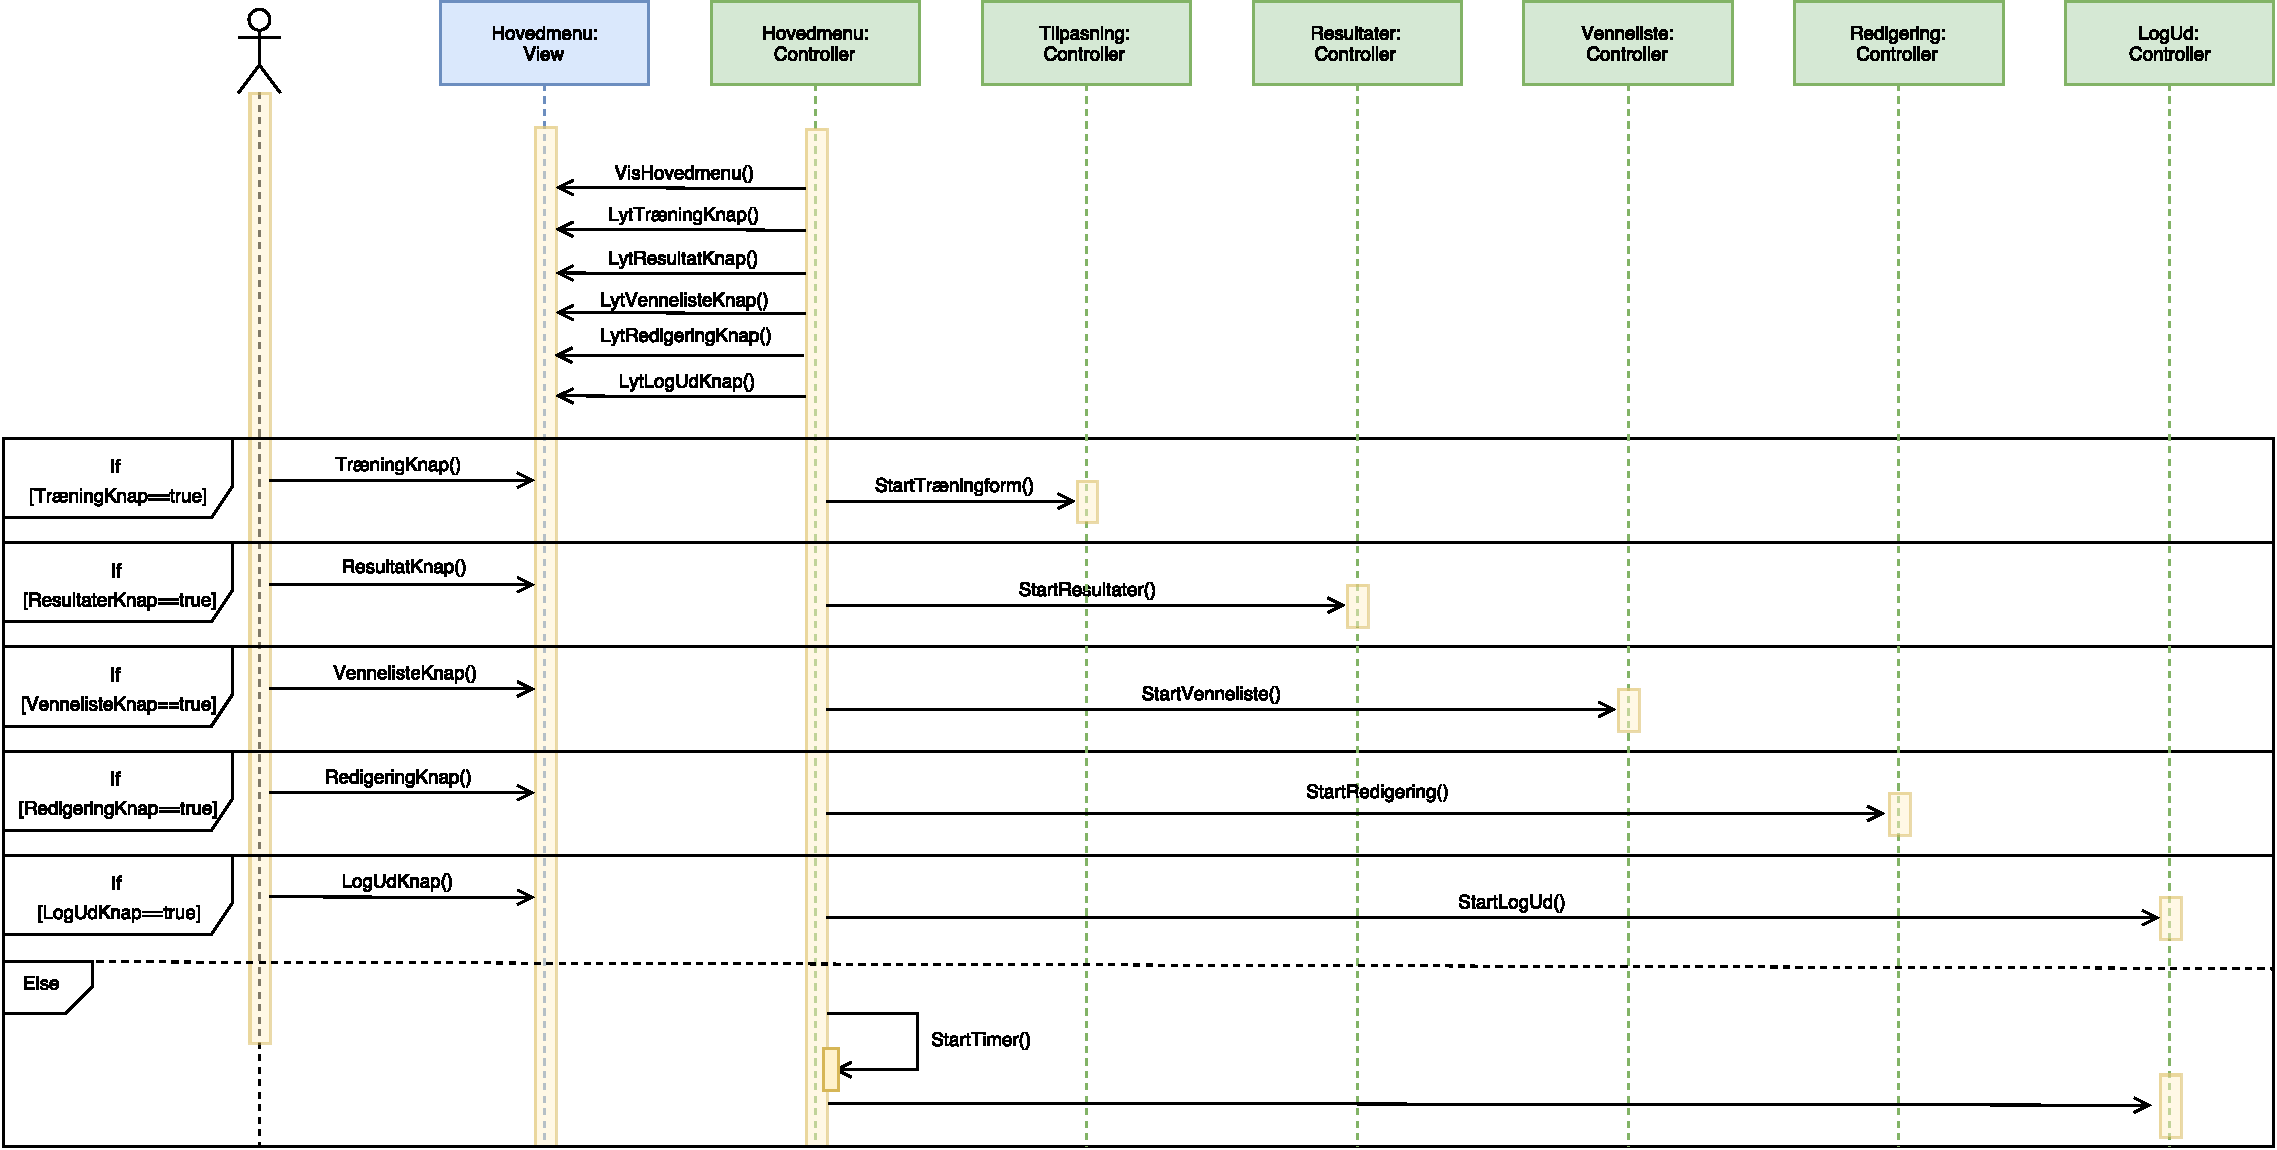
\includegraphics[width=1.5\textwidth, angle=90]{figures/Sek/SEKHovedmenu}
\caption{Sekvensdiagram for hovedmenu. \fxnote{OBS! Hvad skal vi gøre med de forskellige knapper uden eller inden for loop?}}
\label{fig:SEKHovedmenu}
\end{figure}

\noindent
Det fremgår af sekvensdiagrammet, at der er opstillet forskellige if-loops, som viser sekvensen for hver sin knap. Når brugeren angiver sin ønskede funktion, henvises systemet til den dertilhørende controller. Hvis ingen af de opsatte knapper angives, forbliver brugeren på grænsefladen for \textit{Hovedmenuen}, hvorefter en timer starter. 